Two Python array packages existed before NumPy.
The Numeric package began in the mid-90s and provided an array object in
Python, written in C, and linking to standard fast implementations of linear
algebra.
Around 2000, the Space Telescope Science Institute (STScI) software group wrote
a reimplementation of much of Numeric, called NumArray, to support their work
on large memory-mapped arrays and arrays of mixed data type
records \cite{STScI-slither}.
This briefly caused the two communities to diverge, until
2005, when NumPy emerged as a ``best of both worlds'' unification of Numeric
and NumArray \cite{oliphant2006guide}.

Today, NumPy underpins almost every Python library that does scientific or
numerical computation including SciPy \cite{virtanen2019scipy},
Matplotlib \cite{hunter2007matplotlib}, pandas \cite{mckinney-proc-scipy-2010},
scikit-learn \cite{pedregosa2011scikit}, and
scikit-image \cite{vanderwalt2014scikit}.
It is a community developed, open source library, which provides a
multidimensional Python array object along with array-aware functions
that operate on it.
Because of its inherent simplicity, the NumPy array is
the {\it de facto} exchange format for array data in Python.
The library has such widespread adoption that not only the array object but also its
{\it Application Programming Interface} (API) has become ubiquitous as
a language for array programming.

\section*{NumPy arrays}

\begin{figure*}
  \centering
  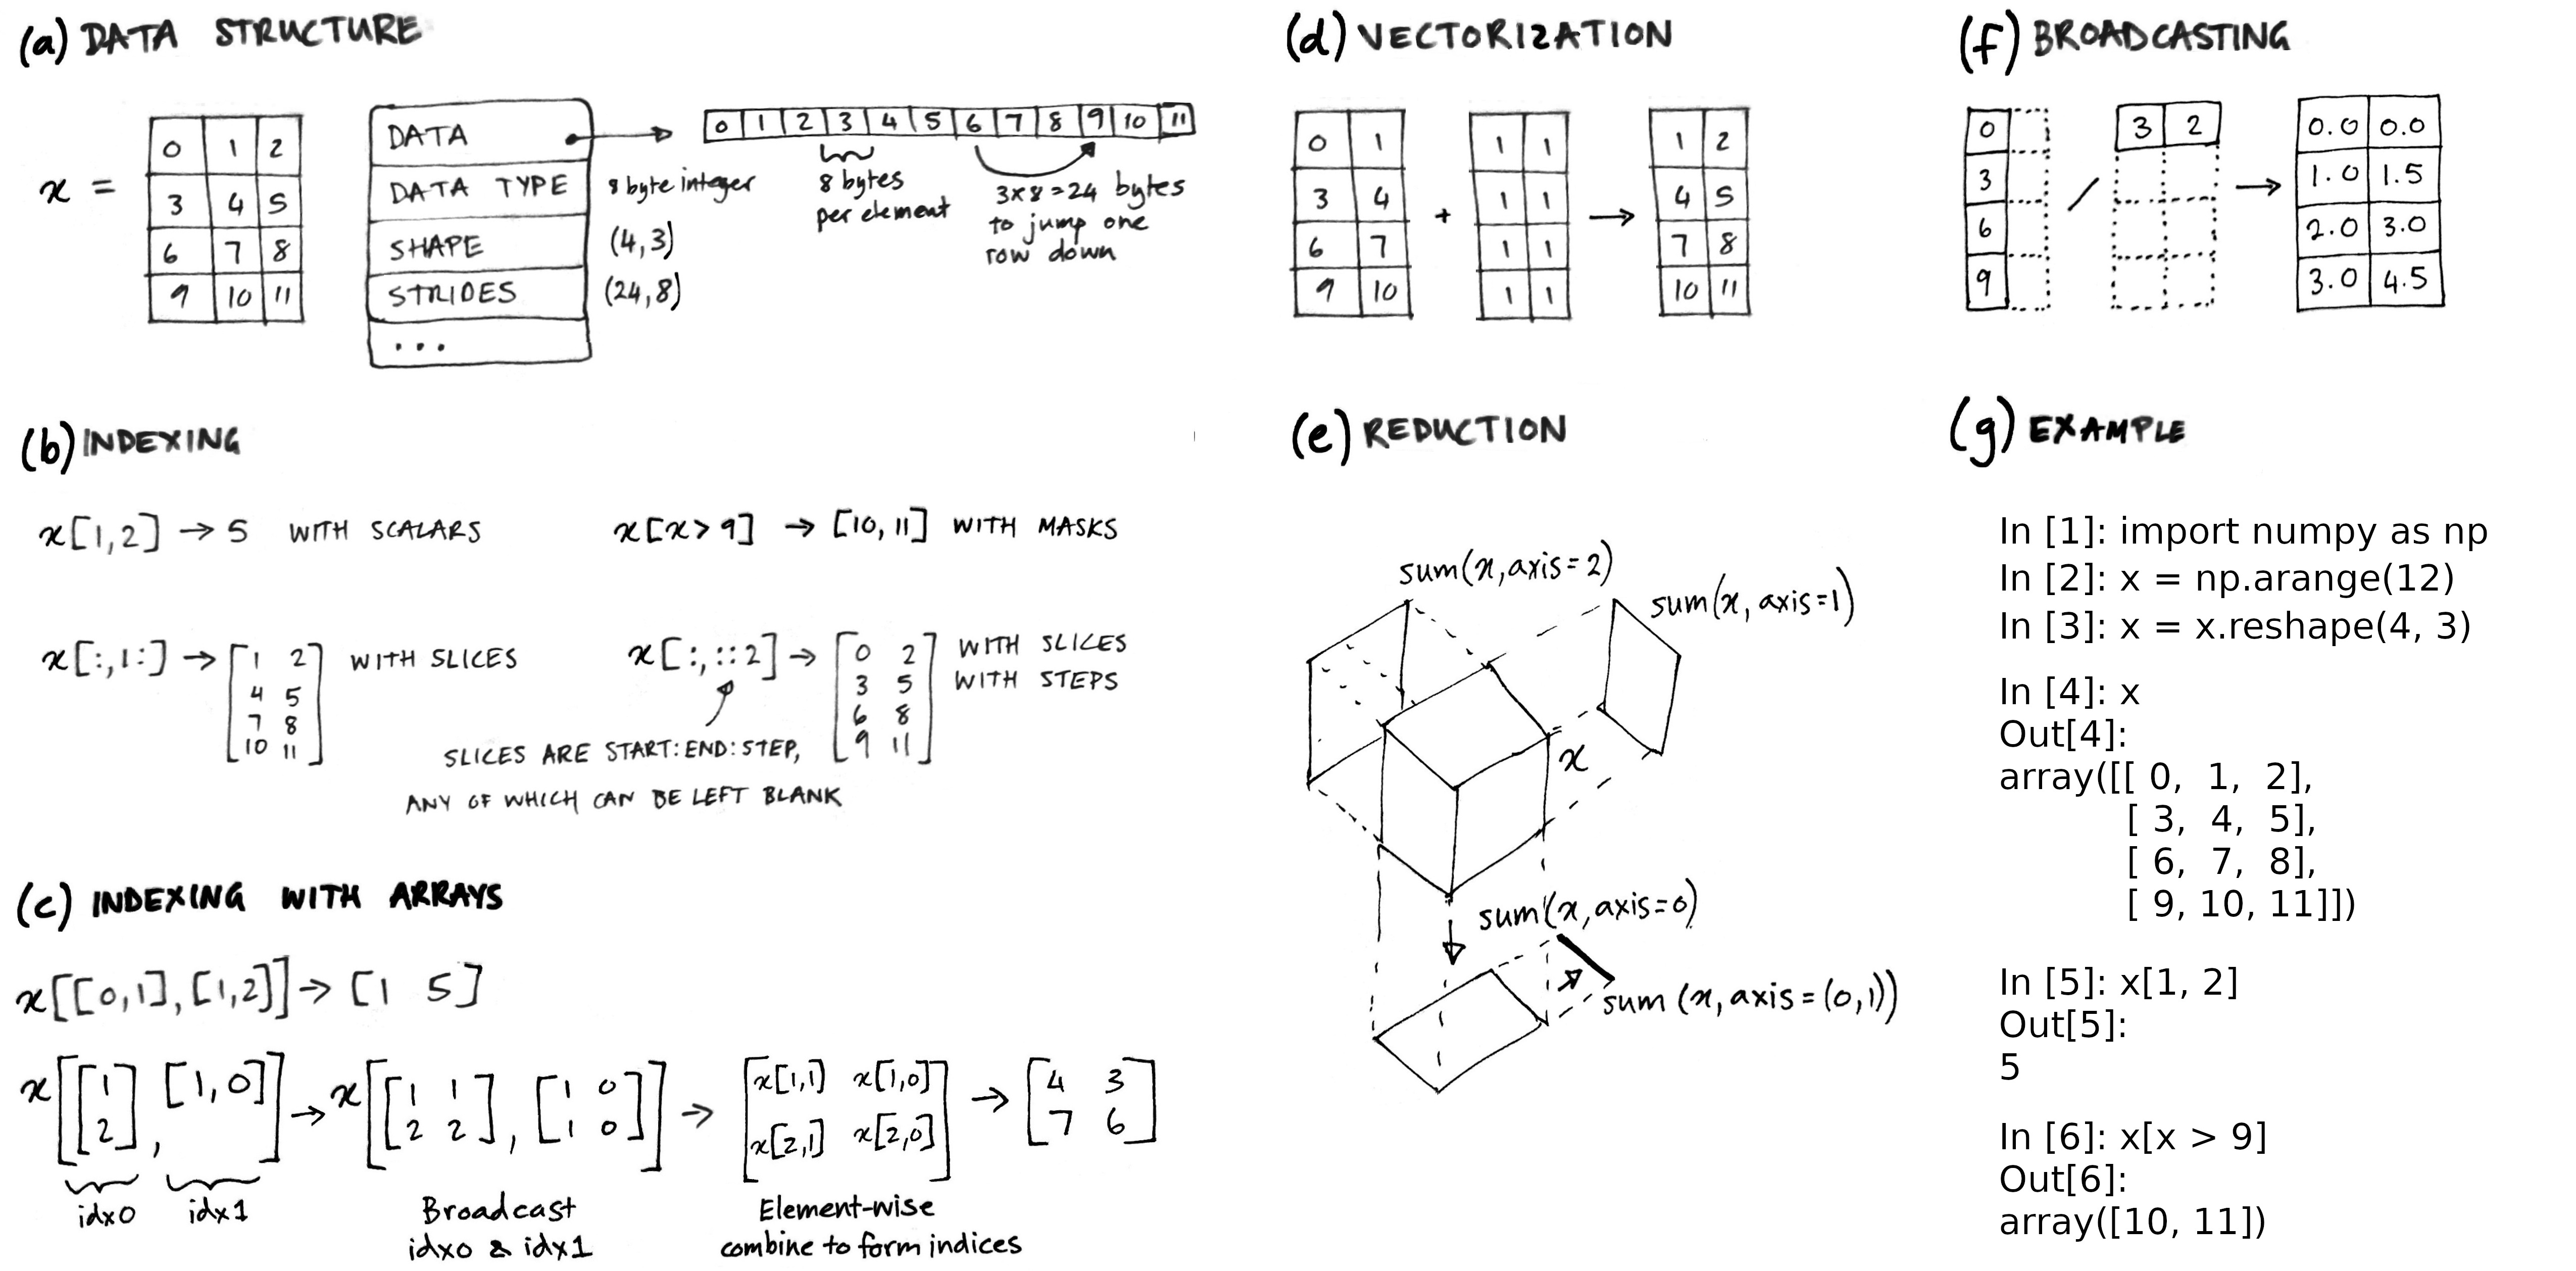
\includegraphics[width=\textwidth]{static/sketches/array-concepts}   
  \caption{\textbf{Fundamental Array Concepts.}
    \textbf{a,} The NumPy array data structure and its associated metadata fields.
    \textbf{b,} Indexing an array with various types of arguments.
    \textbf{c,} Indexing with arrays, which broadcast the indexing arguments before performing the lookup.
    \textbf{d,} Broadcasting in scalar addition, and in the division of two-dimensional arrays.
    \textbf{e,} Reduction operations act along one or more axes. In this
    example, a three-dimensional array is shown to be summed along various single
    axes to produce two-dimensional results, or along two axes consecutively to
    produce a one-dimensional result.
   }
  \label{fig:array-concepts}
\end{figure*}

The NumPy array is a data structure that efficiently stores and accesses
multidimensional arrays \cite{vanderwalt2011numpy}, also known as tensors, that
enables a wide variety of scientific computation.
It consists of a pointer to memory, along with metadata used to interpret the
data stored there, notably {\em data type}, {\em shape}, and {\em strides}
(Fig.~\ref{fig:array-concepts}a).

The {\em data type} describes the nature of elements stored in an array.
n array has a single data type, and each array element occupies the same
number of bytes in memory.
Examples of data types include real and complex numbers (of lower and higher
precision), strings, timestamps, and pointers to Python objects.

The {\em shape} of an array determines the number of elements along each axis,
and the number of axes is the array's dimensionality.
For example, a vector of numbers can be stored as a one dimensional array of
shape $N$, while color videos are four dimensional arrays of shape
$(T, M, N, 3)$.

{\em Strides} are necessary to interpret computer memory, which stores elements
linearly, as multidimensional arrays.
It describes the number of bytes to move forward in memory to jump from row to
row, column to column, and so forth.
Consider, for example, a 2-D array of floating point numbers with shape
$(4, 3)$, where each element occupies 8 bytes in memory.
To move between consecutive columns we need to jump forward 8 bytes in memory,
and to access the next row $3 \times 8 = 24$ bytes.
The strides of that array are therefore $(24, 8)$.  NumPy is able to
store arrays in either C or Fortran memory order, iterating
first over either rows or columns.  This allows external libraries
written in those languages to directly access NumPy array data in memory.

To manipulate the data structure in an intuitive manner, we provide users with
a simple yet powerful array expression syntax.
It supports operations such as indexing (selecting subarrays) and elementwise
calculations.
A high level syntax allows users to express themselves succinctly, while NumPy
deals with the underlying mechanics of making operations fast.

Indexing an array returns single elements, subarrays, or elements that satisfy
a specific condition (Fig.~\ref{fig:array-concepts}b).
Arrays can even be indexed using other arrays (Fig.~\ref{fig:array-concepts}c).
Wherever possible, indexing that retrieves a subarray returns a {\em view} on
the original array, such that data is shared between the two arrays.
This provides a powerful way to operate on subsets of array data, while
limiting memory usage.

A powerful array feature that affects the way NumPy indexes and combines
arrays, is {\em broadcasting}.
When performing an operation (such as addition) on two arrays, one intuitively
expect that these arrays should be required to have the same shape.
However, through broadcasting, NumPy allows the dimensions to differ, while
still producing results that appeal to intuition.
A trivial example is the addition of a scalar value to an array, but it also
generalizes to more complex examples such as scaling each column of an array,
or generating a grid of coordinates.
In broadcasting, one or both arrays are virtually duplicated (that is, without
copying any data in memory), so that the shapes of the operands match
(Fig.~\ref{fig:array-concepts}d).
Broadcasting is also applied whenever an array is indexed using arrays of
indices (Fig.~\ref{fig:array-concepts}c).

To complement the array syntax, NumPy includes functions that perform
elementwise calculations on arrays, including arithmetic, statistics, and
trigonometry.
They aim to loop over array elements near-optimally, taking into consideration,
e.g., strides, in order to best utilize the computer's fast cache memory.
Vectorized operations that would take many tens of lines to express in
languages such as C can often be implemented as a single, clear Python
expression.

Many of these functions, such as summation, support reductions: aggregating
results across one or more dimensions of the array.
For example, summing a $n$-dimensional array over $d$ axes results in a
$(n-d)$-dimensional array (Fig.~\ref{fig:array-concepts}e).

Other array-aware functions include creating, reshaping, concatenating, and padding
arrays; searching, sorting and counting data; and reading and writing files.
NumPy provides extensive support for generating pseudorandom numbers and
includes an assortment of probability distributions.
It also performs accelerated linear algebra, utilizing one of several backends
such as OpenBLAS \cite{wang2013augem,xianyi2012model} and Intel MKL optimized for the CPUs at hand.

\section*{Supporting the ecosystem}

\fixme{Maybe some wording around the actual *support* element?}

% - review supporting the ecosystem (actual support element)
%   - docstrings / testing / packaging
%   - coordinating mechanism
%     - deprecation policy

Users predominantly interact with NumPy arrays using {\em indexing} (to access
subarrays or individual elements), {\em operators} (e.g., $+$, $-$, $\times$,
and, for matrix multiplication, $@$), as well as {\em array-aware functions};
together, these provide an easily readable, expressive, high-level API for
array programming.

Various libraries build on and extend this functionality to further enrich the
ecosystem of available tools.  For example, SciPy adds various mathematical,
scientific, and engineering routines; Pandas provides indexed arrays, known as
dataframes; xarray implements arrays with labeled axes; and Matplotlib
generates publication-ready figures and visualizations.  Employing these
low-level array-aware functions are widely used technique-specific libraries,
including scikit-learn (machine learning), scikit-image (image processing),
statsmodels (statistics),  networkx (graphs and complex networks)
\cite{SciPyProceedings_11}, and Napari (volumetric image visualization).

Finally, domain-specific libraries and applications are built on this diverse
foundation of tooling; these include Astropy (astronomy) \cite{astropy:2013,
astropy:2018}, Biopython (computational biology and bioinformatics) \cite{cock2009biopython},
NIPY (neuroimaging) \cite{millman2007analysis}, and Pangeo (earth science) \cite{2018EGUGA..2012146H}.

Exposing array programming primitives, as well as the surrounding ecosystem of
tools, in Python---an interpreted language---creates an ideal environment for
interactive, exploratory data analysis where users may iteratively inspect,
manipulate, and visualize their data \cite{perez2007ipython}.

\section*{The proliferation of arrays}

\fixme{Add references somewhere to Zarr, https://arrow.apache.org/,
https://parquet.apache.org/,
https://github.com/ruby-numo/numo-narray/wiki/Comparison-with-Numpy}

Recent years have seen a massive explosion in data science, machine learning,
and artificial intelligence.  NumPy and its API, underlying almost every tool
in the computational toolchain, has become ubiquitous.  Still, NumPy itself
could never hope to satisfy every single specialized need of the community; it
is limited in its ability to work with very large datasets, datasets split
across multiple systems, and computations that require specialized hardware.
Furthermore, pursuing solutions to these challenges is out of scope for NumPy
development.

The community's efforts to fill the resultant gaps therefore led to a
proliferation of arrays including distributed arrays---which are stored on
multiple computers, GPU arrays---which utilize graphics processing units for
fast computation, computation graphs---which postpone and combine calculations
before executing them efficiently, and sparse arrays---which typically contain
few non-zero values, and store only those in memory.
%distributed arrays, GPU arrays, delayed execution arrays, sparse arrays,
%foreign language arrays, and more.

\section*{Extensibility and Interoperability}

Given the proliferation of array implementations, a widespread adoption of the
NumPy API remains valuable: it lowers the barrier to entry for newcomers, and
provides the wider community with a stable array programming interface.

What can NumPy do to support the use of its API without blocking innovation?
We believe that having NumPy as a central point of coordination between array
objects can improve interoperability while supporting growth of a larger
surrounding ecosystem of specialized solutions and new tools.  Primarily, there
exist two types of Python array objects: subclasses of NumPy arrays, and arrays
that mimic NumPy arrays but are fundamentally different.

Subclasses of NumPy often exist due to difficulty in constructing richer data
types, such as quantities with physical units \cite{astropy,Goldbaum2018,pint},
geometrical objects \cite{pygeos}, and missing numbers.
To improve \emph{extensibility}, we are currently overhauling the data type
system to make it easier to implement data types both in Python and C, and to
support these and other applications.

There has been a steady increase in the number of external libraries that
provide arrays and a NumPy-like API for manipulating them.
This includes popular tensor computation libraries such as
CuPy\footnote{\url{https://cupy.chainer.org/}},
JAX\footnote{\url{https://jax.readthedocs.io/en/latest/jax.numpy.html}}, and
Apache MXNet\footnote{\url{https://numpy.mxnet.io/}}.
PyTorch\footnote{\url{https://pytorch.org/tutorials/beginner/blitz/tensor\_tutorial.html}}
and
Tensorflow\footnote{\url{https://www.tensorflow.org/tutorials/customization/basics}}
provide tensor APIs with NumPy-inspired semantics.
Ideally, operating on these arrays using NumPy would simply work, so that end
users could write code once, and would then benefit from switching between
NumPy arrays, GPU arrays, distributed arrays, and so forth, as appropriate.

\begin{figure}
  \centering
  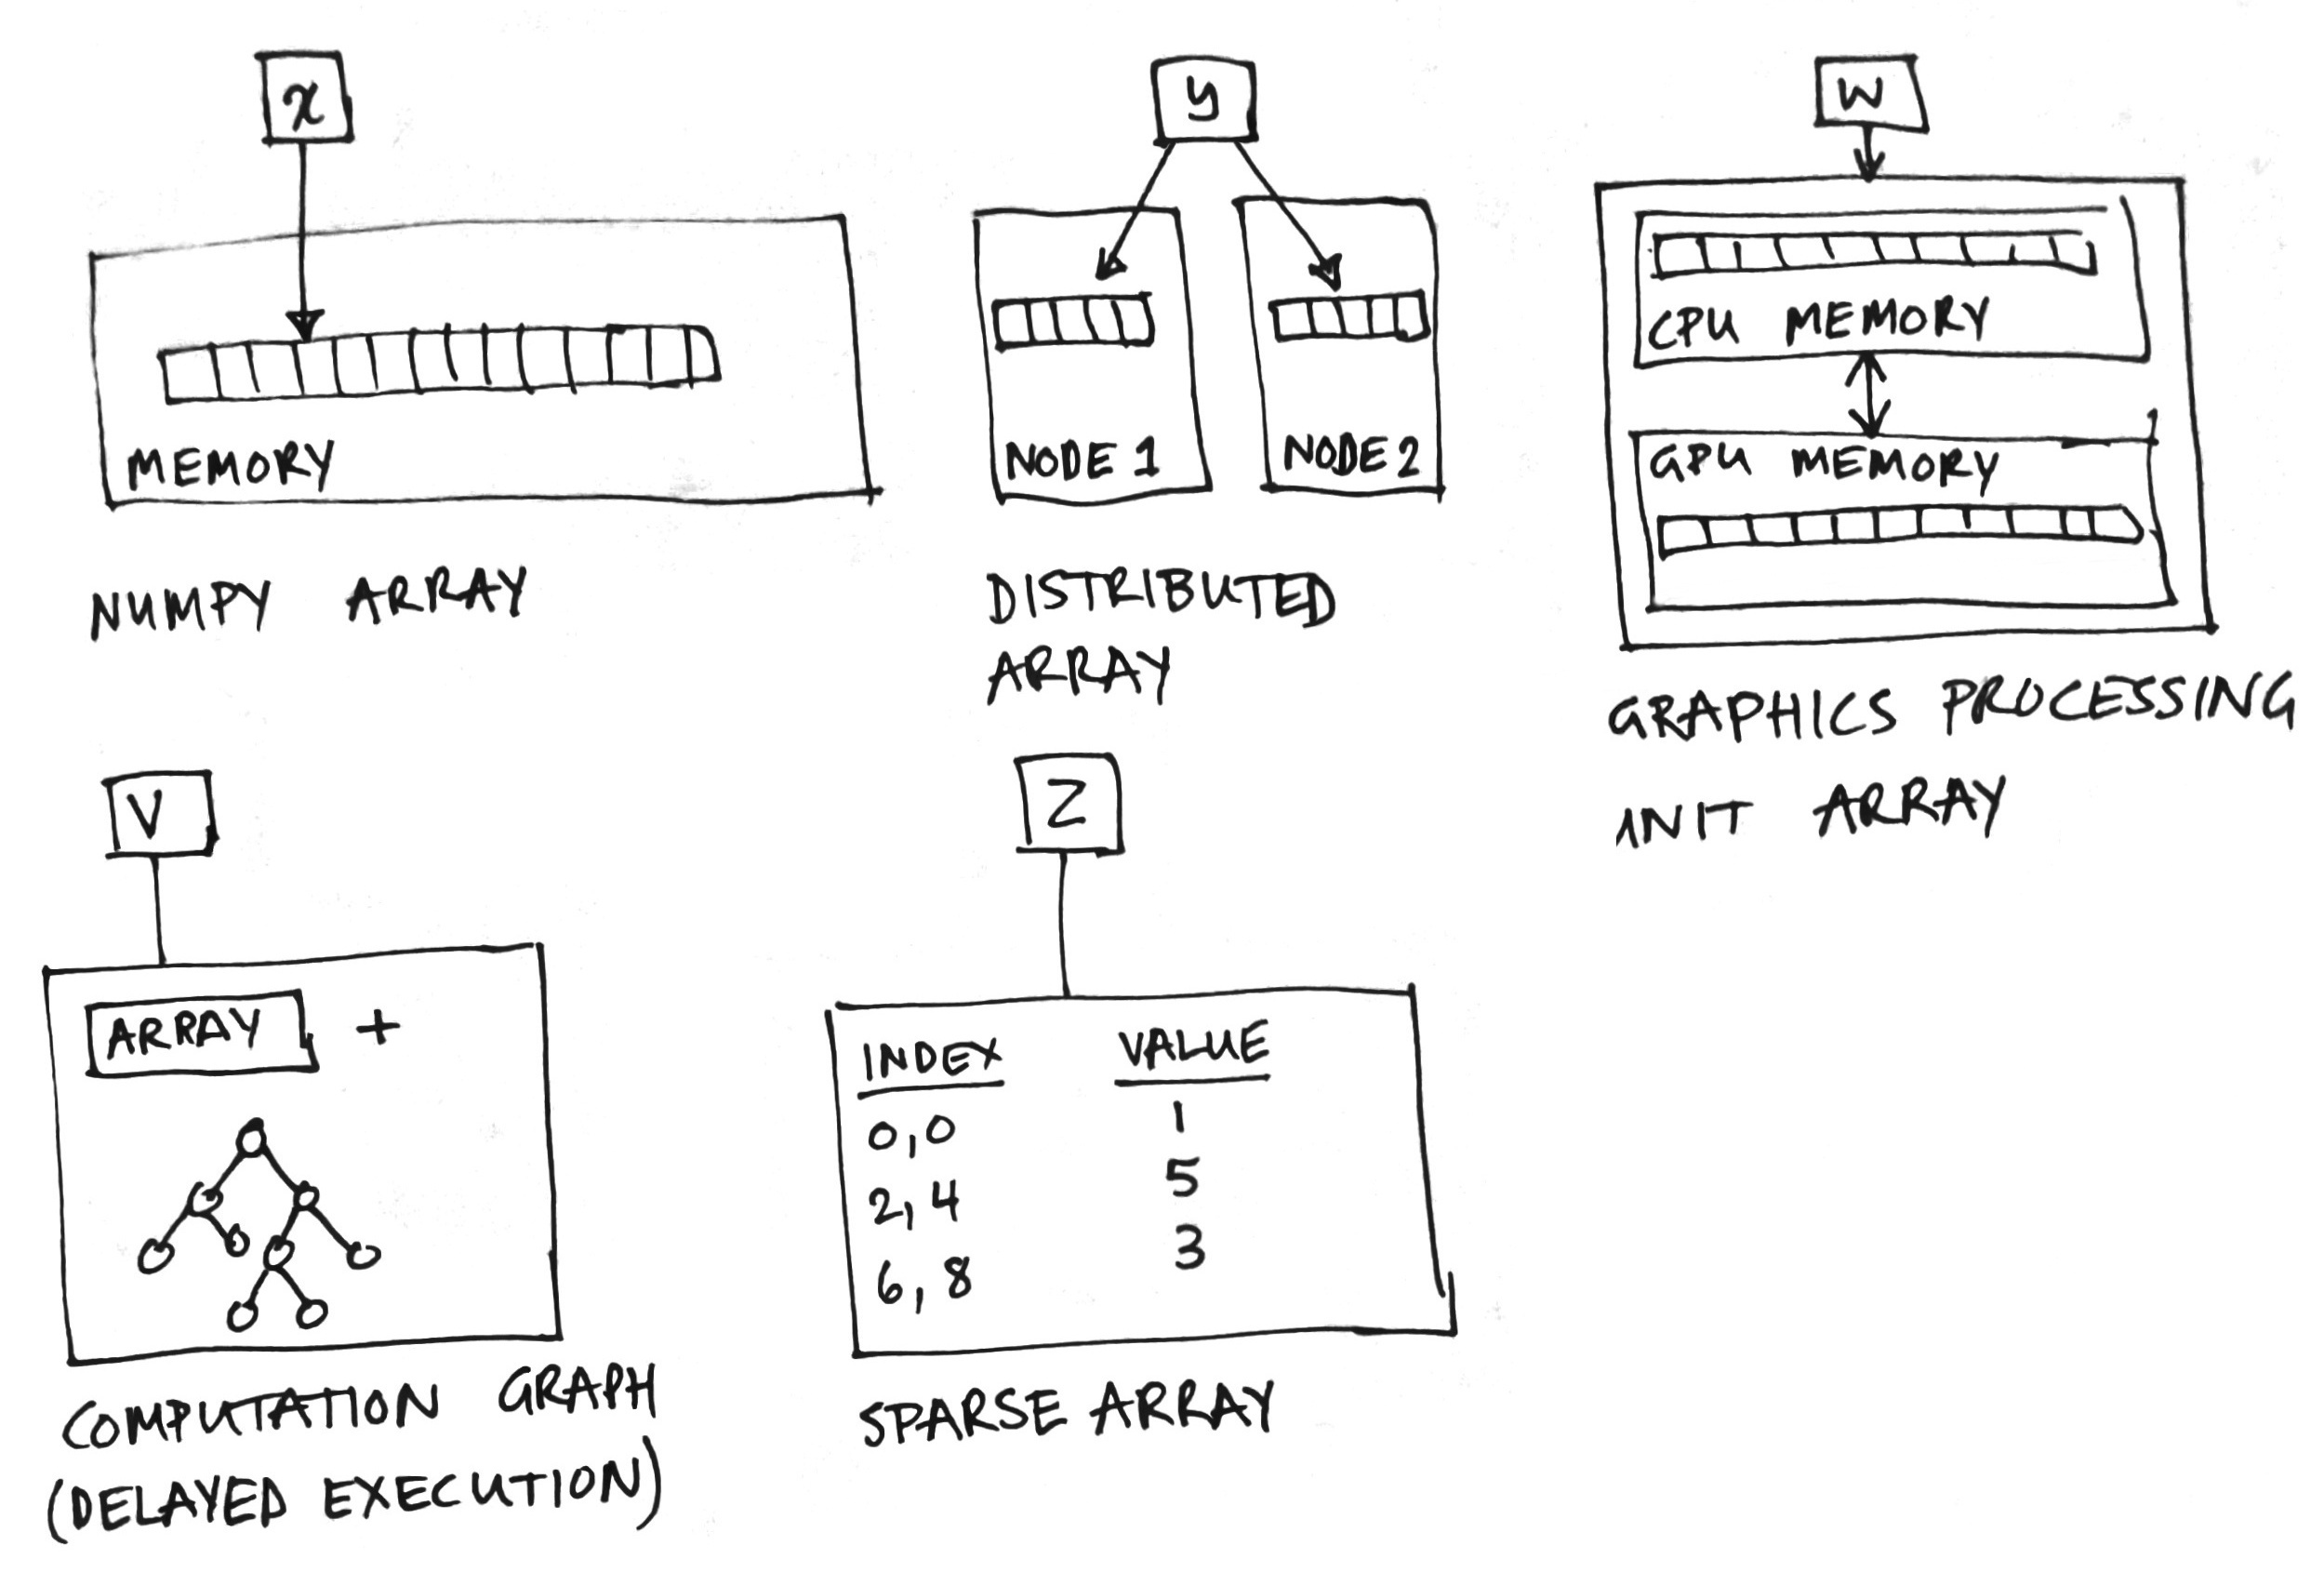
\includegraphics[width=.45\textwidth]{static/sketches/duck-arrays}
  \caption{\textbf{Interoperability.} \fixme{This figure needs work.}}\label{fig:duck-arrays}
\end{figure}


To facilitate \emph{interoperability}, the NumPy team has designed
``protocols'' (or contracts of operation), that allow for these arrays to be
passed to NumPy functions (Fig.~\ref{fig:duck-arrays}).
NumPy, in turn, dispatches operations to the originating library, as required.
% FIXME: expand to 3 or more sentences discussing current efforts and
% issues with those, how did adoption go, what is being done next
%\url{https://numpy.org/neps/nep-0037-array-module.html}
Versions of these protocols have been successfully deployed.
% Ralf: Could you provide some proof of effectiveness, e.g., "This has made it
% possible to create distributed GPU arrays, enabling .... [find a reference to
% work by Peter Entschev]".

% https://numpy.org/neps/nep-0016-abstract-array.html
% https://numpy.org/neps/nep-0018-array-function-protocol.html
% https://numpy.org/neps/nep-0022-ndarray-duck-typing-overview.html
% https://numpy.org/neps/nep-0030-duck-array-protocol.html
% https://github.com/numpy/numpy/blob/a111b551ae940d7d5f8523fef1cf3589c6ba00a0/doc/neps/nep-0033-extensible-dtypes.rst
% https://numpy.org/neps/nep-0037-array-module.html

\section*{Discussion}

% aka why is this so successful
% some sense of ongoing work / future directions

NumPy was initially developed by students, faculty, and researchers in their
spare time to provide a modern array programming library for Python.  They were
influenced by their experiences with powerful interactive programming languages
for scientific computing like Yorick \cite{munro1995using} as well as
commercial languages and environments like IDL and Matlab.  They also
frequently developed code from scratch to solve their own or their colleagues'
problems, often in low-level languages that preceded Python like Fortran
\cite{dongarra2008netlib} and C.

% Fortran / C
% A few sentences on the history of array programming, referencing APL and Fortran, are missing.

NumPy spurred the development of the larger scientific Python ecosystem and
heralded the current era of wide-spread use of Python for scientific computing.
There were several factors that allowed this rapid growth and successful
development.

Python is already a good choice for standard programming tasks such as
cleaning data, interacting with web resources, and parsing text.
It has a wide range of libraries for different tasks.
Adding fast array operations and linear algebra allows the scientist to do all
their work with within the same language---and one that has the advantage of
being famously easy to learn and teach.

NumPy has strong culture of using software engineering practice to
improve collaboration and reduce error \cite{millman2014developing}.
The NumPy team was early in adopting distributed revision control and code
review to improve collaboration on code, and continuous testing that runs a
large battery of automated tests for every proposed change to NumPy.
The project has comprehensive, high-quality documentation, integrated with the
source code \cite{vanderwalt2008scipy,harrington2008scipy,harrington2009scipy}.

% https://ras.ac.uk/sites/default/files/2020-01/Group%20Award%20-%20Astropy.pdf
% https://ras.ac.uk/news-and-press/news/leading-astronomers-and-geophysicists-honoured-ras-bicentenary-year-0

This culture of using best practices for producing reliable scientific software
has been eagerly adopted by the ecosystem of libraries that build on NumPy.
For example, in a recent award given by the Royal Astronomical Society to
Astropy, they state:
\begin{quotation}
\noindent\emph{The Astropy Project has provided hundreds of junior scientists
with experience in professional-standard software development practices
including use of version control, unit testing, code review and issue tracking
procedures. This is a vital skillset for modern researchers that is often
missing from formal university education in physics or astronomy.}
\end{quotation}
Community members explicitly work to address this lack of formal education
through formal courses and workshops
\cite{wilson-software-carpentry,hannay-scientific-software-survey,millman2018teaching}.
%\fixme{cite https://scipy-school.org/}.

Lastly, NumPy benefited greatly from the simplicity of its underlying data
structure, which made it a natural standard for exchanging array data between
libraries.  It also made it easy for other libraries to develop fast and
memory-efficient compiled code, usually in C or Fortran, that could manipulate
these arrays and pass them back to Python.

Over time, and with the arrival of different technologies and array types, the
role of NumPy has changed from merely being an array provider, to being a
widely adopted array programming language.

% S:
%
% Thinking about enabling factors, I'd characterize them into three categories:
%
% - Practical
% - Philosophical
% - Social
% - Technical
%
% E.g., practical: reason why we use Python (learn one language for
% everything); students don't have money, so want to avoid impracticalities of
% license dongles/servers, etc.
%
% Philosophical: science should be open, transparent; our software should be
% controlled by scientists, not designers that we don't have access to
%
% Social: joy of building these things together, friendly welcome into the
% community for many of us---appreciation of our work and hours
